\documentclass{article}
\usepackage[left=2cm,right=2cm,top=1cm,bottom=1cm,a3paper]{geometry}
\usepackage{pgfplots}
\usepackage{parskip}
\usepackage{caption}
\usepackage{multicol}
\usepackage{wrapfig}

\usepackage{float}
\restylefloat{table}

\setlength{\parindent}{0mm}

\pgfplotsset{compat=1.15}

\newcommand{\cia}[1]{\resizebox{\textwidth}{!}{\input{#1}}}
\newcommand{\ciapdf}[1]{\vspace*{-\parskip}\resizebox{0.75\textwidth}{!}{\includegraphics[width=0.75\textwidth]{#1}}}
\newcommand{\halfhalf}[2]{\begin{multicols}{2}\includegraphics[width=0.5\textwidth]{#1} \includegraphics[width=0.5\textwidth]{#2}\end{multicols}}

\begin{document}

\title{Supervised learning task 1}
\author{Lin Zhao (16010906)}
\date{\today}
\maketitle

\newpage

\subsection*{Introduction}

The dataset used for this task is from Schularick and Taylor(2012,
``Credit Booms Gone Bust''). It is an annual dataset covering 14
countries and 140 years. Among the variables they collected, the most
important one is the yearly aggregate bank loans, which is 
the main soure of prediction power. The variable of interest is the
CrisisST which take a value of 1 when there is a financial crisis and 0
otherwise.

Following the guidance of Schularick and Talor(2012), I explored the
relationships between several macro variables within two
eras of finance capitalism, tested the predicting power of different
macro variables, and compared predicting power of different supervised
learning methods. The last part of above is also inspired by the
Fricke(2017, Financial Crisis Prediction: A Model Comparison``). 

The methods used in this part are logistic regression, classification
tree, classification forest, and SVM. The major criteria
used here is area under receiver operating curve. The secondary creteria
is confusion matrix. The major validation method is the modified cross
validation method mentioned in the Fricke paper that take time into
consideration.

\subsection*{Data description and cleaning}

To explore the changing features between two eras, firstly I created
variables of interest: credit to GDP ratio, bank asset to GDP ratio,
money to GDP ratio, credit to money ratio, and bank asset to money
ratio. To see the distinctive trends in different historical periods, I
regroup the whole dataset by years and take mean value of each variable
each year. Ploting mean values of the ratios above against time, I
recovered Figure 1 and 2 in Schularick and Taylor(2012).

Figure 1 shows that bank loans, bank asset and broad money supply remain
steady related to the size of economy representing by GDP,
before the WW2 period. After the war, the money to GDP ratio stays flat
while the other two start to increase dramatically. In figure 2 we
can see that the loan to money ratio and bank asset to money ratio start
to take off after the distruction of WW2 implying that credit start to
grow faster than broad money supply and no steady relationship between
the too can be found in this period.

\ciapdf{Figure_1.pdf}

\ciapdf{Figure_2.pdf}

To study financial crisis caused by the economy system, we need to
exclude the crisis caused by the two world war. As did in Schularick and
Taylor paper, I excluded the war period(1914 to 1919 and 1939 to 1947)
and German crisis after WW1(1920 to 1925). Divided the cleaned up
dataset into pre- and post-war period, I recovered the upper panel of
table 1 in the paper.

\subsection*{Annual summary statistics pre- and post-war}

\begin{table}[H]
    \begin{tabular}{|l|l|l|l|l|l|}
    \hline
          & credit\_to\_GDP & bankAsset\_to\_GDP & money\_to\_GDP & credit\_to\_money & bank\_asset\_to\_money \\ \hline
    count & 685             & 611                & 736            & 662               & 580                    \\ \hline
    mean  & 0.408977        & 0.714051           & 0.533292       & 0.735337          & 1.282481               \\ \hline
    std   & 0.359888        & 0.447337           & 0.207534       & 0.449343          & 0.566104               \\ \hline
    \end{tabular}
\end{table}

\begin{table}[H]
    \begin{tabular}{|l|l|l|l|l|l|}
    \hline
          & credit\_to\_GDP & bankAsset\_to\_GDP & money\_to\_GDP & credit\_to\_money & bank\_asset\_to\_money \\ \hline
    count & 831             & 828                & 834            & 833               & 831                    \\ \hline
    mean  & 0.546975        & 1.013497           & 0.645801       & 0.838012          & 1.575839               \\ \hline
    std   & 0.423878        & 0.668770           & 0.240497       & 0.494226          & 0.752540               \\ \hline
    \end{tabular}
\end{table}

More than half of the countries in the dataset are from
Europe, so I also excluded all the observations in post WW1 period(1920 to
1925) since all the crises happened in
that period could be caused by WW1 rather than economical system. I also
dropped any row that contains missing value. I
only kept the variables that have protentially strong prediction power
according to the results and the robustness test from the paper.

After cleaning, I have 1433 observations and 59 out of these are crisis
events.

\subsection*{Supervised learning methods for classification}

\subsubsection*{Logistic regression and choice of explanatory variables}

As defined in Schularick and Taylor paper, I created cpi nomalized bank
loan and take the difference of log value of this variable as the change
of credit environment. This variable will be called credit change. I also
take credit to GDP ratio as one protential
explanatory variable base on robustness test of the paper. This variable
lagged 1 year will be called credit size. After
assign each country for each year its lagged 1 to 5 credit change, I
sorted the dataset by time to make sure that when fitting a model, it is
not trying to predict 1960s crisis with 1990s' data.

I started the analysis by useing lag 1 to lag 5 diff-log credit to fit a
logistic regression model. The AUC is slightly higher than 0.5 for the whole
dataset and for the pre-war dataset, and significantly higher than 0.5
for the post-war dataset. Since in the paper, lag 2 credit change is the only lagged variable that
is significant, I also fitted logistic regression with only lag 2 data
and the model fit slightly better for both whole set and pre-war period
in respect of AUC. The change in post-war period is umbiguous and 
credit size seems add prediction power to the post-war period. The lag 2 credit change is indeed the
main sourece of information.

\subsubsection*{In-sample AUC for logistic regression with lag 2 credit change}

\begin{table}[H]
    \caption{in-sample logistic regression trained with wholde time period,
    pre-war period and post war period with lag 2 credit change as major
    explanatory variable.}
    \begin{tabular}{|l|l|l|l|}
    \hline
                        & whole set          & pre-war            & post-war           \\ \hline
    without credit size & 0.6373277827336704 & 0.6286424526999033 & 0.697533908754624  \\ \hline
    with credit size    & 0.4518906730102092 & 0.5177922018137459 & 0.7200369913686806 \\ \hline
    \end{tabular}
\end{table}

I did a out-of-sample test for the choice of variable using
30\% of the dataset as test set and 70\% as training set.
The result show that model fitted with lag 2 credit change have
significantly better out-of-sample performance than model fitted with
lag 1 to lag 5 and credit size doesn't seem to add predicting
power to the model. The AUC are reported in the following tables.

\subsubsection*{Out-of-sample AUC for logistic regression with lag 1 to lag 5 credit change}

\begin{table}[H]
    \caption{out-of-sample logistic regression trained with 70\% of
    each data set and tested on 30\% of data with lag 1 to lag 5
    credit change as major explanatory variable.}
    \begin{tabular}{|l|l|l|l|}
    \hline
                        & whole set          & pre-war            & post-war           \\ \hline
    without credit size & 0.5861360718870345 & 0.5762987012987013 & 0.7608543417366948 \\ \hline
    with credit size    & 0.5892169448010269 & 0.5800865800865801 & 0.615546218487395  \\ \hline
    \end{tabular}
\end{table}


\subsubsection*{Out-of-sample AUC for logistic regression with lag 2 credit change}

\begin{table}[H]
    \caption{
    table 5: out-of-sample logistic regression trained with 70% of
    each data set and tested on 30% of data with lag 2 credit change
    as major explanatory variable.
    }
    \begin{tabular}{|l|l|l|l|}
    \hline
                        & whole set          & pre-war            & post-war           \\ \hline
    without credit size & 0.7370988446726572 & 0.7976190476190476 & 0.7461484593837535 \\ \hline
    with credit size    & 0.531193838254172  & 0.6737012987012987 & 0.6355042016806722 \\ \hline
    \end{tabular}
\end{table}

\ciapdf{Figure_4.pdf}
\begin{quote}
Figure 4: out-of-sample AUC of logistic model fitted with 70% of
data as training set and 30% as testing set. All three period
fitted with lag 2 credit change only.
\end{quote}

Given result above, I only considered lag 2 credit change and credit
size variable. This also means all the model compared here will have
same information as input and thus makes the comparison meaningful.

At last for logistic regression, I did a modified cross validation
mentioned in the Fricke paper. I divided the wholde dataset in to four
equal folds. First, I use fold one to train and test on fold two. Then I
use fold one and two to train and test on fold three, etc.. The average
AUC is 0.56129 which is higher than 0.5. The reason for divide the
dataset into 4 rather than 5 fold like did in the Fricke paper is that
when the fold is too small, due to the sparseness of crisis events,
there might be only one class in the whole training set or test set.

\subsection*{Tree and forest}

Next I fitted the data with a classification tree. With maxmum depth
equals to 3, here are result of in-sampel prediction. It is obvious from
the table that credit size add on predicting power for classification
tree at least for in-sample test.

\subsection*{AUC for classification tree}

\begin{table}[H]
    \caption{
    in-sampel classification tree fitted with lag 2 credit change
    as major explanatory variables
    }
    \begin{tabular}{|l|l|l|l|}
    \hline
                        & whole set          & pre-war            & post-war           \\ \hline
    without credit size & 0.6937568143522649 & 0.7030106338903466 & 0.780209617755857  \\ \hline
    with credit size    & 0.7598684210526315 & 0.7878746029553929 & 0.8358199753390876 \\ \hline
    \end{tabular}
\end{table}

From the AUC plot we can see that there are much less point on each line
for the tree compared with logistic regression. This is because for
logistic regression, each observation will have its own estimated
probability, but for a tree, the observation belong to the same leaf
will have the same probability.

\ciapdf{Figure_5.pdf}
\begin{quote}
Figure 5: AUC of classification tree fitted with whole time period,
pre-war and post-war period. All three period fitted with lag 2 credit
change and credit size.
\end{quote}

For the choice of maxmum depth, we need a good balance between fully use
all the information and avoid over fitting. To find the maxmum depth
that gives highest AUC for each tree, I performed an analysis with
following steps: 1\textgreater{} for each of whole set, pre-war, and
post-war period, set up a modified cross validation of 5 fold as
mentioned in logistic regression part with certain maxmum depth and
record the average AUC for each model. 2\textgreater{} collect average
AUC of each model for maxmum depth from 2 to 50. 3\textgreater{} plot
the average AUC against maxmum depth for each model and pick up the
depth that coincide with the highest AUC.

\ciapdf{Figure_6.pdf}
\begin{quote}
Figure 6: Average AUC for the whole, pre- and post-war dataset fitted
with and without credit size plot against maxmum depth
\end{quote}

With optimal max-depth 3, 3, 5 respectlly, I fitted 70\% training set of whole period and
pre-war dataset with lag 2 credit change and post-war with lag 2 credit
change and credit size. With 30\% of the total data as a test set, these models show AUC 0.62895,
0.69021 and 0.43697 respectlly.

The dramatically different performance between in-sample and
out-of-sample test is caused by over fitting. Given a high enough
max-depth, classification tree can acheive AUC 1.0 in an in-sample test.
But over fitting will lead to very poor out-of-sample prediction. This
is indicated by the flatening out in the figure above. Two trees with different maxmum depth in the appendex demonstrate
this point.

With exactly same idea, I performed analysis with classification forest
model. The in-sample performance is better than the tree with same
max-depth which could either caused by higher predicting power or
overfitting.

\subsection*{AUC for classification forest}


\begin{table}[H]
    \caption{in-sampel classification forest fitted with lag 2 credit change
    as major explanatory variable.}
    \begin{tabular}{|l|l|l|l|}
    \hline
                        & whole set          & pre-war            & post-war           \\ \hline
    without credit size & 0.7419033105362275 & 0.7823735211526954 & 0.9169852034525278 \\ \hline
    with credit size    & 0.7619994548518189 & 0.8678359342632234 & 0.8669852034525277 \\ \hline
    \end{tabular}
\end{table}

\ciapdf{Figure_7.pdf}
\begin{quote}
Figure 7: AUC of classification forest fitted with whole time period,
pre-war and post-war period. First two period fitted with lag 2 credit
change and credit size and post-war fitted with lag 2 credit change
only.
\end{quote}

With optimal max-depth picked up by the same method as in the tree
analysis, datasets are fitted with lag 2 credit change and/or credit
size. Tested with 30\% data in the dataset, the AUC are 0.62426,
0.73593, and 0.71709 for whole, pre-war and post-war data.

Tree and forest learners perform brilliantly in-sample and
are not much more impresive than logistic regression in out-of-sample test. Forest
perform slightly better than tree method.

In both tree and forest analysis, I used gini index and entropy and
there are little difference between the AUC.

\subsection*{SVM}

When fitting SVM model with the data, I used two kinds of kernels:
rbf(Gaussion kernel) and sigmoid kernel. The results are both affected
by randomness when fitting the model and sigmoid kernel in general has
better out of sample perfomance. 


\subsection*{A few interesting facts and potential explanations}


When taking a closer look to the results of tree and forest, I found a
few interesting facts. First, for both tree and forest, I found the
results are different when fitting models with exactly same data set and
parameters, indecating randomness in the
fitting precesure. Second, for the
model fitted with both lag 2 credit change and credit size, the average
AUC show fluctuation in the over fitting tail. In the plot of forest,
all model show fluctuation in the over fitting tail parts but for models
with two explainory variables, the fluctuations have higher amplitude.
Last, for some trees and forests, the out
of sample AUC do not drop to 0.5 even in the obviously over fitting
zone.

To answer the first question, one need to identify the souce of
randomness. I found two protential sources for tree and three for
forest by reading the document. One obvious candidate is the random start point when searching
for the optimal arguments to minimize cost function. However, as long as
the problem is convex, the searching reslults should be with in a
relatively small intervel with possible difference due to limited resolution. This
doesn't match the observation. An argument
called max\_features in tree is defined as``The number of features to consider when
looking for the best split(sklearn.tree.DecisionTreeClassifier document
page)''. When fitted with two variables, the model with max
feature setted to 1 shows jumps while model with max features setted to 2 does not. For the forest, there is one extra
source of randomness. To grow multiple trees, the sklearn library
bootstrap observations using random selection with replacement. In both tree and forest sklean
function, the argument random state controls all the
randomness.

Carrying knowledge mentioned above, I try to decompose the fluctuations.
Fixing random state eliminates fluctuation in
AUC-max-depth plot of both treee and forests. For the forest, I first turn off the max
feature limit, and the resulting plot doesn't show less fluctuation.
Next, I add the limit on max feature and turn off bootstrap, and
this reduced the fluctuation. And eventually, when I turn off both limit
and bootstrap, the fluctuation was almost totally eliminated. These
changes indicates that the
forest fitting is extremely sensitive to the chang of training dataset.
Another interesting observation here is that the AUC of model fitted
with pre-war data and with both credit change and credit size as
explainory variables dropped below 0.5 benchmark after the limit and
bootstrap was turn off. I cannot explain this change. Relavent plots are in the appendix.

I notice that the model that has
prediction power even when over fitted are models fitted with the whole
dataset. This is ture for both tree and forest analysis(with
randomness turn off in forest). From the plot of AUC of trees fitted
with different datasets, I notice that there is only one point in each
of the three line. This indecates that in the out of sample test, only
the first split take effect, most likely due to
over fitting. The whole set has the largest number of observations, it is likely that
even when over fitted, the first split has some predicting power. Here
is one exampel of AUC plot when over fitted. This also explains the same
observation in the forest analysis.

\ciapdf{Figure_11.pdf}
\begin{quote}
Figure 11: All three models are fitted with lag 2 credit change and
credit size. These models are fitted with 80% of dataset and
tested on 20% of set. To eliminate effect of randomness, the
ramdom state argument was fixed when fit these models.
\end{quote}

\subsection*{Another criteria}

Except for AUC, confusion matrix is also a good criteria for model
comparison. In the tables below, I collected full out-of-sample results for logistic
regression and forest fitted with 70\% of whole data set regarding confusion matrix. False alarm is defined as
M01 / (M01 + M11), and can be interpreted as when model say crisis, how much of that are
miss classified. Total flag is the percentage of total observation that has been flagged by the model as crisis.

To capture 10\% of the crisis,
logistic regression need to flag 2\% of the total observation, and 80\%
of those flags are false alarm. On the other hand, forest need only flag
less than 1\% of data and only half of those are false alarm. However,
if the goal is to capture half of the crisis, logistic regression only
need to flag less than 20\% of data with 87\% false alarm while forest
need to flag half of the data point and more than 90\% of the flag are
false alarm. The main idea here is that there is no sigle best criteria
and the criteria selection should be based on the goal of analysis.

\begin{multicols}{2}
\begin{table}[H]
        \caption{Out-of-sample performance for logistic regression based on confusion matrix.
        Logistic regression fitted with 70\% of the whole period and
        tested with 30\% of whole period. Explanory variable is lag 2
        credit change only. AUC is 0.73709.}
        \begin{tabular}{|l|l|l|l|}
        \hline
         threshold         & sensitiveity        & falseAlarm         & totalFlag            \\ \hline
        0.95845 & 0.05263 & 0.87500              & 0.01865 \\ \hline
        0.95842 & 0.10526 & 0.80000                & 0.02331 \\ \hline
        0.95829 & 0.15789 & 0.80000                & 0.03497  \\ \hline
        0.95817 & 0.21053 & 0.84000               & 0.05828  \\ \hline
        0.95814 & 0.26316  & 0.83333 & 0.06993  \\ \hline
        0.95805 & 0.31579  & 0.86047 & 0.10023  \\ \hline
        0.95801 & 0.36842  & 0.86000               & 0.11655  \\ \hline
        0.95799 & 0.42105 & 0.85185 & 0.12587   \\ \hline
        0.95796 & 0.47368 & 0.85714 & 0.14685  \\ \hline
        0.95793 & 0.52632  & 0.87179 & 0.18182  \\ \hline
        0.95791 & 0.57895  & 0.88172 & 0.21678  \\ \hline
        0.95790 & 0.63158   & 0.88119 & 0.23543  \\ \hline
        0.95789 & 0.68421  & 0.88288 & 0.25874  \\ \hline
        0.95786 & 0.73684  & 0.89313 & 0.30536  \\ \hline
        0.95773 & 0.78947  & 0.92823 & 0.48718  \\ \hline
        0.95767 & 0.84211  & 0.93701  & 0.59207   \\ \hline
        0.95764   & 0.89474  & 0.93885 & 0.64802   \\ \hline
        0.95759 & 0.94737  & 0.94098  & 0.71096    \\ \hline
        0.95745 & 1.00000                 & 0.95000               & 0.88578   \\ \hline
        \end{tabular}
\end{table}

\begin{table}[H]
        \caption{Out-of-sample performance for forest based on confusion matrix. Forest fitted with 70\% of the whole period and tested on
        30\% of the whole period. Variable is lag 2 credit change only,
        max depth is 3. The AUC of this model is 0.67079.}

    \begin{tabular}{|l|l|l|l|}
    \hline
     threshold           & sensitiveity        & falseAlarm         & totalFlag            \\ \hline
    0.31088  & 0.05263 & 0.00000                & 0.00233 \\ \hline
    0.15587  & 0.10526 & 0.50000                & 0.00932 \\ \hline
    0.05381   & 0.15789 & 0.90909 & 0.07692  \\ \hline
    0.04785 & 0.36842  & 0.89394 & 0.15385  \\ \hline
    0.04160  & 0.73684  & 0.93665 & 0.51515   \\ \hline
    0.03808  & 0.84211  & 0.93822 & 0.60373   \\ \hline
    0.03177  & 0.89474  & 0.93885 & 0.64802   \\ \hline
    0.01070 & 0.94737  & 0.95000               & 0.83916   \\ \hline
    0.00829  & 1.00000                 & 0.95571 & 1.00000                  \\ \hline
    \end{tabular}
\end{table}
\end{multicols}

\subsection*{Conclusion and potential further questions to answer}

In this study, I implemented
a few supervised learning models on the data. The major predicting
power lies in lag 2 credit change and this conclusion alines with
Schularick and Taylor paper. Prediction power of models are much stronger in sample. This confirms the result of Fricke
paper. Tree and forest are particularly
vulnarable to over fitting thus require carefully picked parameters like
maxmum depth or maxmum number of leaves. They are also quite sensitive
to the change of training set. Another issue for
tree and forest is that when there is a dominating class in the training
data, there model generated could be biasd. This issue can be reduced by
balance the data prior fitting or assign similar weight to different
classes. However, these are not explored in this report and can be
interesting topic for futher study. Since forest shows great protential
to predict crisis, and machine learning methods are not widly use in
economical research, solving this issue may have practical meaning. All
the models tested in this report show some level of predicting power.
However, there is no single standard to judge which is the best model.
The selecting criteria strongly depends on the purpose of the analysis
and different models may have adventages in different tasks.

\begin{thebibliography}{9}
\bibitem{booms} 
Moritz Schularick \& Alan M. Taylor
\textit{Credit Booms Gone Bust: Monetary Policy, Leverage Cycles, and Financial Crisis, 1870-2008}.

\bibitem{fcp} 
Daniel Fricke
\textit{Financial Crisis Prediction: A Model Comparison}.
\end{thebibliography}

\section*{Appendix}

Figure 1: nomal depth tree

\ciapdf{app_normaldepth.pdf}

Figure 2: over fitting tree 

\vspace*{-\parskip}\resizebox{\textwidth}{!}{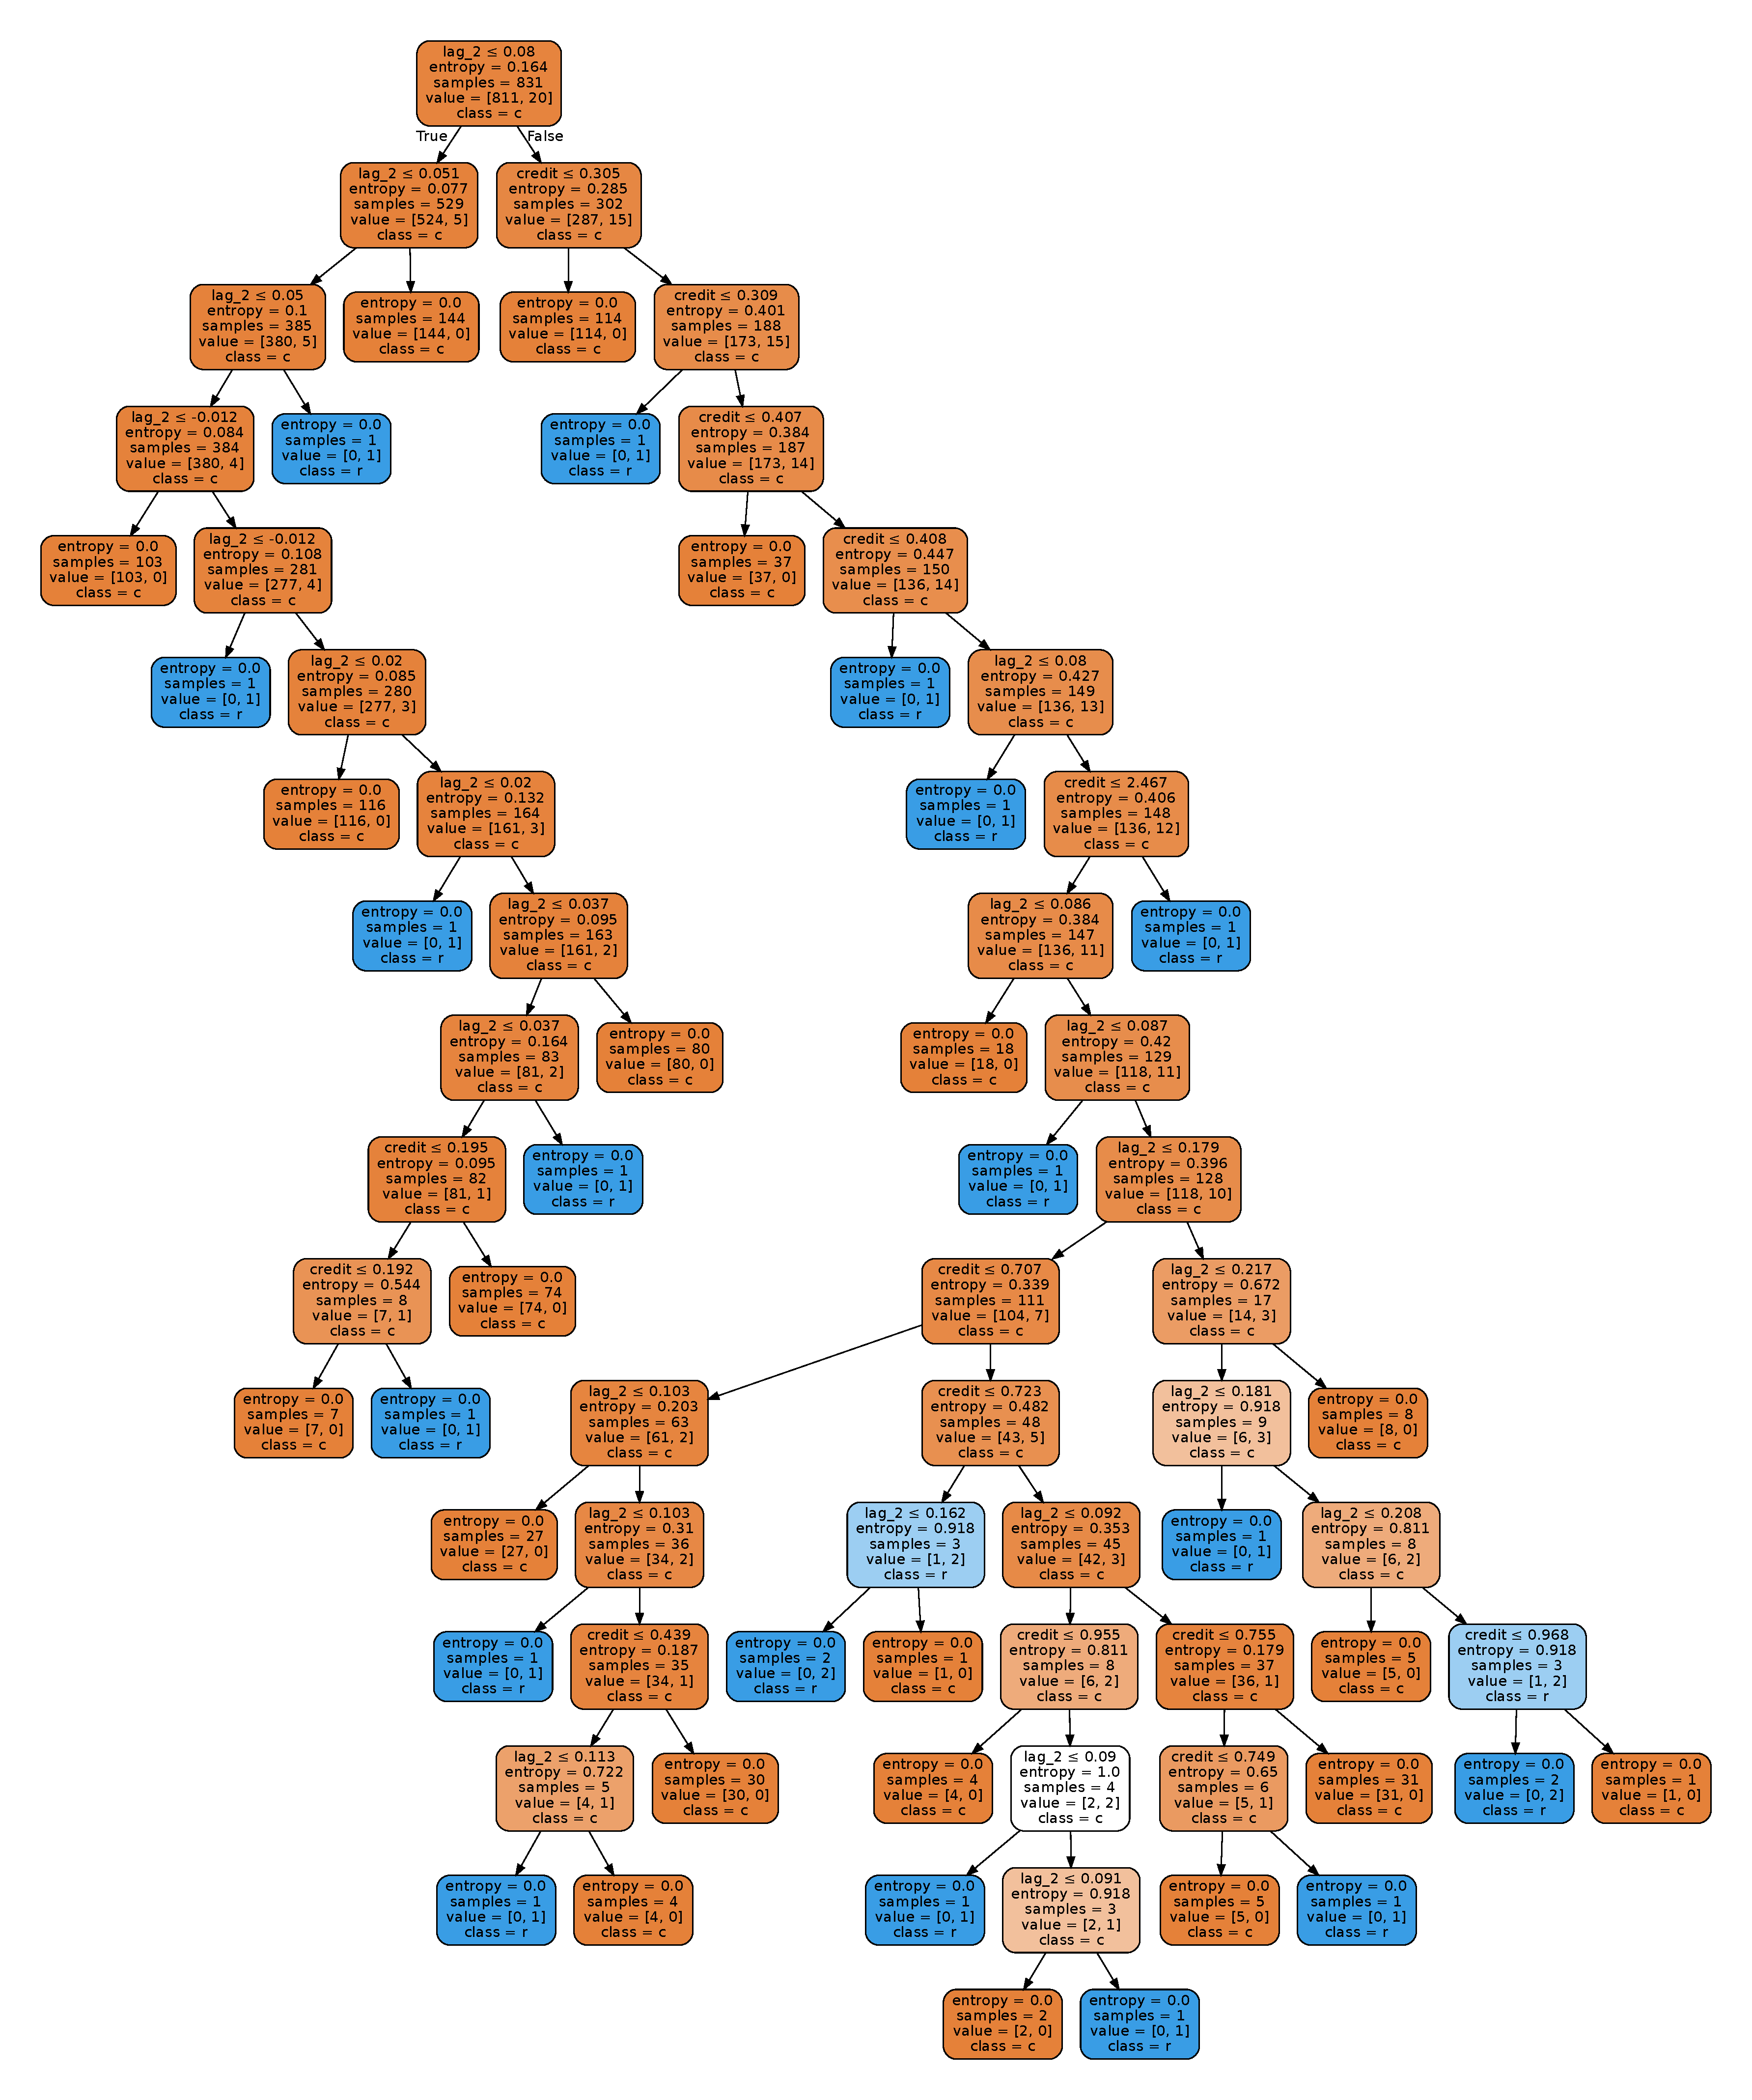
\includegraphics{app_overfitting.pdf}}

Figure 3:
different trees generated by same data with limited max feature

\ciapdf{app_samedata_1.pdf}

\ciapdf{app_samedata_2.pdf}

\ciapdf{Figure_8.pdf}
\begin{quote}
Figure 8: The maxmum feature is limited and bootstrap is on, this is
exactly the same plot used to choose optimal depth. We can see a lot of
fluctuation here at least three AUC do not approach 0.5 benchmark.
\end{quote}

\ciapdf{Figure_9.pdf}
\begin{quote}
Figure 9: The maxmum feature is limited and bootstrap is off, and we can
see that fluctuation is reduced.
\end{quote}

\ciapdf{Figure_10.pdf}
\begin{quote}
Figure 10: The maxmum feature is unlimited and bootstrap is off, and we
can see dramatical reduce of fluctuation and only two lines do not
approach 0.5 benchmark.
\end{quote}


\end{document}
